

\section{Ejercicio 1: Filtro notch pasivo}
\subsection{C\'alculo te\'orico}
\subsubsection{Dise\~no de los componentes}
Para el c\'alculo te\'orico se consider\'o al circuito como dos cuadripolos en paralelo, de los cuales se obtuvieron sus par\'ametros admitancia.
El primero de los cuadripolos es el presentado en la figura \todo[inline]{INSERT REFERENCE TO FIGURE Q1}.
\missingfigure{First quadrupole circuit}
El c\'alculo de los par\'ametros viene facilitado por la simpleza del circuito y el hecho de ser rec\'iproco, de forma que sus par\'ametros admitancia son:

\begin{align}
    \label{eqn: Admittance parameters first quadrupole.}
    y_{A11} = \left. \frac{I_1}{V_1} \right\rvert_{V_2=0} = \frac{1}{R_1 + \frac{R_2}{R_2 \cdot C_3 \cdot s + 1}} = \frac{R_2 \cdot C_3 \cdot s + 1}{R_1 \cdot R_2 \cdot C_3 \cdot s + \left(R_1+R_2\right)} \\
    y_{A12} = \left. \frac{I_1}{V_2} \right\rvert_{V_1=0} = \frac{-I_2 \cdot \frac{1}{R_1 \cdot C_3 \cdot s + 1}}{I_2 \cdot \left(R_2 + \frac{R_1}{R_1 \cdot C_3 \cdot s + 1}\right)} = -\frac{1}{R_1 \cdot R_2 \cdot C_3 \cdot s + \left(R_1+R_2\right)}\\
    y_{A21} = \left. \frac{I_2}{V_1} \right\rvert_{V_2=0} = -\frac{1}{R_1 \cdot R_2 \cdot C_3 \cdot s + \left(R_1+R_2\right)}\\
    y_{A22} = \left. \frac{I_2}{V_2} \right\rvert_{V_1=0} = \frac{R_1 \cdot C_3 \cdot s + 1}{R_1 \cdot R_2 \cdot C_3 \cdot s + \left(R_1+R_2\right)}
\end{align}

De forma an\'aloga se obtienen los par\'ametros para el segundo cuadripolo \todo[inline]{INSERT REFERENCE TO FIGURE Q2}, bas\'andose en los c\'alculos del primero, y tomando provecho de su similitud.
\missingfigure{Second quadrupole circuit}

\begin{align}
    \label{eqn: Admittance parameters second quadrupole.}
    y_{B11} = \frac{\frac{1}{R_3 \cdot C_2 \cdot s} + 1}{\frac{1}{R_3 \cdot C_1 \cdot C_2 \cdot s} + \frac{1}{C_1 \cdot s} + \frac{1}{C_2 \cdot s}} \\
    y_{B12} = -\frac{1}{\frac{1}{R_3 \cdot C_1 \cdot C_2 \cdot s} + \frac{1}{C_1 \cdot s} + \frac{1}{C_2 \cdot s}}\\
    y_{B21} = -\frac{1}{\frac{1}{R_3 \cdot C_1 \cdot C_2 \cdot s} + \frac{1}{C_1 \cdot s} + \frac{1}{C_2 \cdot s}}\\
    y_{B22} = \frac{\frac{1}{R_3 \cdot C_1 \cdot s} + 1}{\frac{1}{R_3 \cdot C_1 \cdot C_2 \cdot s} + \frac{1}{C_1 \cdot s} + \frac{1}{C_2 \cdot s}}
\end{align}

Se observa que la condici\'on de Brune para cuadripolos en paralelo se cumple, y en consecuencia, se obtienen los par\'ametros admitancia del cuadripolo total mediante la suma de sus dos componentes.
Dado que el objetivo final es calcular $\frac{V_o}{V_i}$, como tal cociente solo depende de los par\'ametros $y_{21}$ y $y_{22}$, s\'olo se mostrar\'a el c\'alculo de estos.
Luego de trabajo algebr\'aico, se llega a la siguiente expresi\'on:

\begin{equation}
    H(s) = \frac{V_o}{V_i} = -\frac{y_{A21} + y_{B21}}{y_{A22} + y_{B22}} = \\
\end{equation}

\begin{equation} 
    \label{eqn: Complete transfer function}
    = \frac{R_1 \cdot R_2 \cdot R_3 \cdot C_1 \cdot C_2 \cdot C_3 \cdot s^3 + \left(R_1 + R_2\right) \cdot R_3 \cdot C_1 \cdot C_2 \cdot s^2 + R_3 \cdot \left(C_1 +C_2\right) \cdot s + 1}
    {R_1 \cdot R_2 \cdot R_3 \cdot C_1 \cdot C_2 \cdot C_3 \cdot s^3 + \left(\left(R_1 + R_2\right) \cdot R_3 \cdot C_1 \cdot C_2 + R_1 \cdot R_3 \cdot C_1 \cdot C_3 + R_1 \cdot \left(R_2 + R_3\right) \cdot C_2 \cdot C_3\right) \cdot s^2 + R_3 \cdot \left(C_1 +C_2\right) \cdot s + 1}
\end{equation}

Si se pide que $R_1 = R_2 = 2 \cdot R_3$ y $C_1 = C_2 = \frac{C_3}{2}$ se lleva la expresi\'on de la ecuaci\'on \ref{eqn: Complete transfer function} a:
\begin{equation} 
    \label{eqn: Notch transfer function}
    H(s) = \frac{R_3^2 \cdot C_3^2 \cdot s^2 + 1}{R_3^2 \cdot C_3^2 \cdot s^2 + 4 \cdot R_3 \cdot C_3 \cdot s + 1}
\end{equation}

Se pide que $f_0 = 2,7 KHz$
\begin{equation}
    \implies \omega_0 \approx  16,965 \cdot 10^3 \frac{rad}{s}
\end{equation}

De la ecuaci\'on \ref{eqn: Notch transfer function} se obtiene que:
\begin{equation}
    \omega_0^2 = \frac{1}{R_3^2 \cdot C_3^2} \implies \omega_0 = \frac{1}{R_3 \cdot C_3}
\end{equation}

Debe buscarse alguna combinaci\'on de $R_3$ y $C_3$ que me d\'e $\approx 0,058946 ms$.
La mejor combinaci\'on con valores comerciales es 15 y 39, ya que $15 \cdot 39 = 585$ (luego se corrige el \'orden).
Para la elecci\'on de los componentes se tuvo en cuenta que el \'orden de magnitud de los capacitores sea tal que permita despreciar la capacidad par\'asita de las puntas del osciloscopio, y que adm\'as haya disponibilidad de los componentes en el pa\~nol de la universidad.
Quedan as\'i determinados tambi\'en los valores de $R_1, R_2, C_1$ y $C_2$:
\begin{align}
	\label{eqn: Selection of components}
    R_3 = 1,5 K\Omega \implies R_1 = R_2 = 2 \cdot R_3 = 3 K\Omega \longrightarrow \textrm{ Elijo  } R_1 = R_2 = 3,3 K\Omega \\
    C_3 = 39 nF \implies C_1 = C_2 = \frac{C_3}{2} = 19,5 nF \longrightarrow \textrm{ Elijo  } C_1 = C_2 = 18 nF
\end{align}

Se consider\'o tambi\'en utilizar dos resisencias en serie y dos capacitores en paralelo para lograr exactamente las relaciones indicadas.
Sin embargo, la opci\'on fue descartada por duplicar costo de componentes y, si bien mejora lo esperado en valores nominales, llega a duplicar las tolerancias de las resistencias y capacitores formados por dos componentes.
Consecuentemente, la variaci\'on obtenida en la pr\'actica puede ser a\'un m\'as alejada de los valores esperados.
Finalmente, y como criterio definitivo, se recalcul\'o la variaci\'on de lo esperado al utilizar componentes que no respetan estr\'ictamente la relaci\'on de doble o mitad.
Utilizando la funci\'on transferencia de la ecuaci\'on \ref{eqn: Complete transfer function}, se observa que el coeficiente de grado 3 ser\'a:
\begin{equation}
    f_0 = \frac{1}{2\pi \cdot \sqrt{\left(R_1 + R_2\right) \cdot R_3 \cdot C_1 \cdot C_2}} = \frac{1}{2\pi \cdot \sqrt{\left(3,3 K\Omega + 3,3 K\Omega\right) \cdot 1,5 K\Omega \cdot 18 nF \cdot 18nF}} \approx 2,81 KHz
\end{equation}

Se observa que la variaci\'on es menor al $5\%$ ($4,07\%$ de hecho), dentro de los rangos de tolerancia de los elementos utilizados (todos de $5\%$).
Por lo tanto, se admite el error.



\subsubsection{Caracterizaci\'on del sistema}
Tomando de la expres\'o de la ecuaci\'on \ref{eqn: Notch transfer function}, queda expresada la funci\'on transferencia como:
\begin{equation}
    \label{eqn: Theoretical transfer function with numbers}
    H(s) = \frac{3,475 \cdot 10^{-9} s^2 + 1}{3,475 \cdot 10^{-9} s^2 + 2,358 \cdot 10^{-4} \cdot s + 1}
\end{equation}

Para obtener la respuesta al impulso, se expresa la ecuaci\'on \ref{eqn: Theoretical transfer function with numbers} en fracciones simples:
\begin{equation}
    H(s) = \frac{5248,5}{s+4545,35} - \frac{73104,6}{s+63310,8} + 1
\end{equation}

Y se antitransforma por Laplace:
\begin{equation}
    \label{eqn: Theoretical impulse response}
    h(t) = 5248,5 \cdot \exp{-4545,35 \cdot t} \cdot u(t) - 73104,6 \cdot \exp{63310,8 \cdot t} \cdot u(t) + \delta(t)
\end{equation}

Dado que el sistema es LTI, causal y BIBO-estable, se puede obtener la respuesta en frecuencia realizando el reemplazo $s = j \cdot 2\pi \cdot f$ en la ecuac\'on \ref{eqn: Theoretical transfer function with numbers}:
\begin{equation}
    \label{eqn: Theoretical frequency response}
    H(f) = \frac{f^2 - 7,289 \cdot 10^6}{f^2 - 10799,6 \cdot j \cdot f - 7,289 \cdot 10^6}
\end{equation}



\subsubsection{Respuesta al escal\'on}
Para la obtenci\'on de la respuesta al escal\'on, se realizar\'a primero el producto de la funci\'on transferencia con la transformada de Laplace del escal\'on:
\begin{equation}
    H(s) \cdot U(s) = \frac{1,155}{s+63310,8} -  - \frac{1,155}{s+4545,35} + \frac{1}{s}
\end{equation} 

Antitransformando por Laplace se obtiene que la respuesta al escal\'on es:
\begin{equation}
    \label{eqn: Theoretical response to Heaviside}
    y(t) = 1,155 \cdot \exp{63310,8 \cdot t} \cdot u(t) + 1,155 \cdot \exp{-4545,35 \cdot t} \cdot u(t) + u(t)
\end{equation}

En la cual se puede observar que tendr\'a un m\'inimo. El mismo se obtiene derivando la expresi\'on \ref{eqn: Theoretical response to Heaviside} e igualando a 0:
\begin{align}
    y'(t) = 5248,5 \cdot \exp{-4545,35 \cdot t} - 73104,6 \cdot \exp{63310,8 \cdot t} + \delta(t)\textrm{      para t>0} \\
    y'(t) = 0 \iff t \approx 45 \mu s
\end{align}



\subsection{Simulaci\'on en LTspice}
Para la simulaci\'on del circuito se realizaron dos an\'alisis, ambos del tipo Monte Carlo.
El primero (figura \todo[inline]{REF TO AC ANALYSIS CIRCUIT}), para obtener la respuesta en frecuencia, se logr\'o mediante la herramienta AC Analysis.
El segundo (figura \todo[inline]{REF TO TRANS CIRCUIT}), para obtener la respuesta al escal\'on, se realiz\'o utilizando la herramienta Transient.

\missingfigure{AC ANALYSIS CIRCUIT}
\missingfigure{TRANS CIRCUIT}



\subsection{Resultados experimentales y comparaci\'on con te\'oricos y simulados}
El llevado a la pr\'actica y medici\'on del circuito se realiz\'o a trav\'es de la impresi\'on en PCB del mismo, para el cual se tomaron ciertos criterios explicados a continuaci\'on.
El circuito se aloj\'o en una placa de 5x5cm, simple faz, dado que la simpleza del mismo no ameritaba el uso de dos capas.
Podr\'ia argumentarse que el tama\~no ex excesivo y sobrado para la aplicaci\'on, y se estar\'ia en lo correcto.
Sin embargo, se utilizaron las medidas mencionadas ya que son las m\'inimas disponibles en el pa\~nol de la universidad.
Por otro lado, el cortar la placa habr\'ia supuesto un sobretrabajo innecesario. \\
Se colocaron alojamientos para 4 pines a izquierda y derecha de la placa, para la se\~nal de entrada y salida, respectivamente, tratando de mantener tambi\'en, la simetr\'ia visual del circuito.
De los cuatro pines, solo los dos en los extremos fueron utilizados, quit\'andose los del medio para lograr mayor separaci\'on y prevenirse contra cortocircuitos debidos a la cercan\'ia de los pines.
La conexi\'on con pines se eligi\'o por sobre borneras para facilitar la conexi\'on al generador de se\~nales y a las puntas del osciloscopio.\\
En cuanto a las pistas, se procur\'o que no formasen \'angulos de 90° o m\'as agudos, af\'in de evitar se\~nales par\'asitas por emisi\'on de ondas electromagn\'eticas.
Debido tambi\'en a la disponibilidad de espacio, se le dio a las mismas un ancho de 0,9 mm, facilitando la circulaci\'on de corriente.\\
Finalmente, del lado de la placa sin cobre, se imprimieron las indicaciones de los componentes y los puertos, para facilitar su uso.
Teniendo en cuenta todo esto, el resultado fue el siguiente circuito:
\begin{figure}[h]
    \centering
    \begin{minipage}{\textwidth}
        \centering
        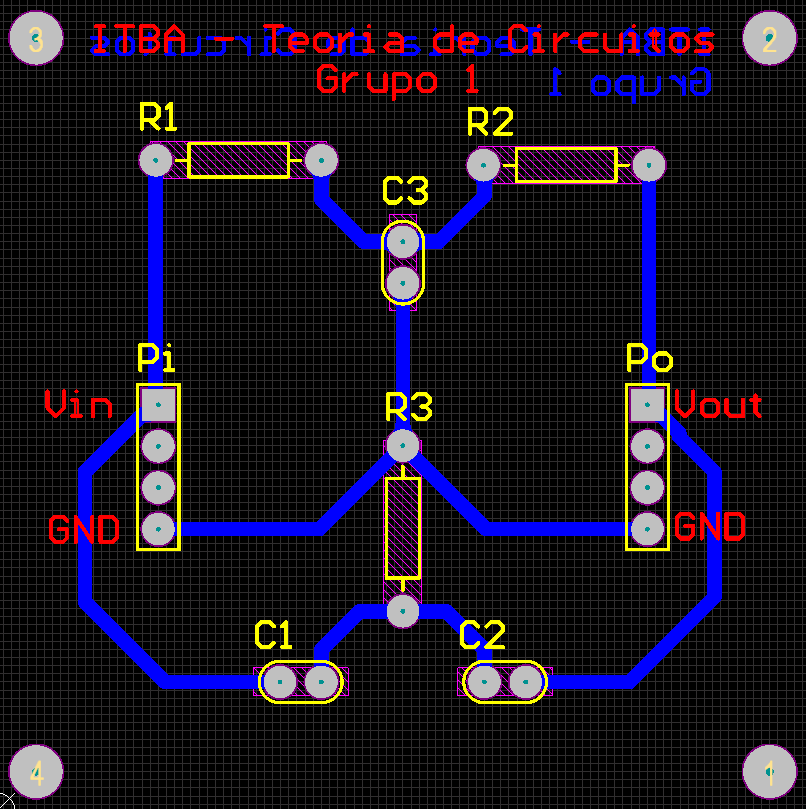
\includegraphics[width=0.7\textwidth]{./EJ1/PCB.png}
        \caption{PCB dise\~nado en el programa Altium Designer.}
        \label{fig: PCB_Altium}
    \end{minipage}\hfill
\end{figure}




\subsubsection{Comparaci\'on de las curvas}
\missingfigure{COMBINATION OF 3 GRAPHS FOR AMPLITUDE BODE}
\todo[inline]{SHORT ANALYSIS OF THE GRAPH}
\missingfigure{COMINATION OF 3 GRAPHS FOR PHASE BODE}
\todo[inline]{SHORT ANALYSIS OF THE GRAPH}
\missingfigure{COMBINATION OF 3 GRAPHS FOR RESPONSE TO HEAVISIDE}
\todo[inline]{SHORT ANALYSIS OF THE GRAPH}